\documentclass[UTF8,a4paper,zihao=-4]{ctexart}

\usepackage[margin=2.25cm]{geometry}
\usepackage{amsmath}
\usepackage{amssymb}
\usepackage{array}
\usepackage{booktabs}
\usepackage{float}
\usepackage{graphicx}
\usepackage{longtable}
\usepackage{multirow}
\usepackage{pgfplots}
\usepackage{tabularx}
\usepackage{xcolor}
\usepackage{tikz}
\usepackage{url}
\usepackage[colorlinks=true,linkcolor=blue!60!black,citecolor=blue!60!black,urlcolor=blue!60!black]{hyperref}

\usetikzlibrary{arrows.meta,positioning,fit,calc,shapes.geometric}
\usepgfplotslibrary{groupplots}
\pgfplotsset{compat=1.18}

\renewcommand{\arraystretch}{1.16}
\newcommand{\code}[1]{\texttt{#1}}
\newcommand{\metric}[1]{\textsc{#1}}

\title{\textbf{MiniMT3-Piano：面向练习与展示场景的钢琴自动音乐转录与谱面生成系统}}
\author{陈昊 \and 覃徐阳}
\date{2026 年 5 月}

\begin{document}

\maketitle

\begin{abstract}
钢琴自动音乐转录旨在从音频中恢复音高、起止时间、力度和踏板等符号信息。已有研究在标准数据集上取得了较高的音符识别指标，但面向练习和展示的转谱系统还需要进一步解决可读谱面生成问题：演奏级 MIDI 中合理存在的细微时值、踏板延音和局部误检，经过机械量化后往往会变成碎休止符、错位和弦和难以阅读的 MusicXML。本文总结 MiniMT3-Piano 的完整系统设计与收束结果。系统从 MT3 风格序列建模探索出发，最终收束到 dense AMT 主线：以 log-mel 表示为输入，使用多头网络预测 onset、frame、offset、velocity 和 duration，并在解码阶段引入 onset-gated 约束、和弦恢复、pitch-aware calibration 和上下文约束的混合修正。系统同时保留演奏 MIDI 和展示谱两个输出目标，将 performance MIDI 到 MusicXML 的处理作为独立谱面层，显式处理量化、分声部、和弦锁定、长音连线和休止符隐藏。实验在固定的 \code{val\_calib512} 与展示曲目上进行。收束结果表明，v15 模型在数值指标与候选音规模之间最平衡，达到 \metric{note-F1}=0.5799、\metric{offset-F1}=0.2880、\metric{pred/ref}=0.956；v19 在 \metric{note-F1} 与 \metric{offset-F1} 上略高，但 \metric{pred/ref}=0.753，存在欠生成，不适合直接用于展示谱；v13 则提供更干净稳定的谱面基底。基于 v13 和 v19 的 hybrid 策略在 Test\_new 展示样例中改善了和弦垂直性，并保持可见休止符较低。本文的贡献在于形成了一套可复现、可诊断、面向谱面展示的钢琴转录系统，并以事件级指标和谱面级指标共同评价其效果。

\noindent\textbf{关键词：}自动音乐转录；钢琴转录；MusicXML；onset-gated 解码；MIDI-to-score；谱面生成
\end{abstract}

\section{引言}

自动音乐转录（Automatic Music Transcription, AMT）试图从音频中恢复可由计算机处理的音乐符号表示。对于钢琴而言，转录系统通常需要同时估计多个声部中大量重叠音符的音高、起始时间、结束时间、力度和踏板状态。近年来，Onsets and Frames 将 onset 检测与 frame 检测联合训练，并在推理时限制新音只能由 onset 触发，使钢琴 AMT 的准确性得到显著提高 \cite{hawthorne2018onsets}。随后，ByteDance 的高分辨率钢琴转录系统通过回归 onset、offset 与踏板时间，在 MAESTRO 数据集上报告了 96.72\% 的 onset F1 \cite{kong2021highres}。MT3 则将 AMT 扩展为多任务、多音轨的序列到序列转录问题，展示了统一建模的潜力 \cite{gardner2022mt3}。

然而，练习与展示场景中的转谱目标并不等同于单一的 AMT 排行榜指标。一个实用的钢琴转谱系统通常包含两个层次。第一层是演奏级转录，即尽量准确地恢复音符事件，输出可听的 MIDI。第二层是谱面级整理，即将演奏事件转化为可阅读、可排版、可展示的 MusicXML。后一任务需要估计拍点、节拍、量化网格、左右手分配、声部分配、连线、休止符和和弦对齐。Score Transformer 和 PM2S 等工作均说明，从 performance MIDI 到可读乐谱本身就是独立问题 \cite{suzuki2021scoretransformer,liu2022pm2s,beyer2024midi2score}。如果直接把 AMT 输出逐音符写入五线谱，系统即使拥有较高 recall，也可能生成大量碎休止符、错位音符和不自然的长音切分。

MiniMT3-Piano 正是在这一实际背景下展开。系统初期参考 MT3 的序列化思路，随后将主线收束为钢琴专用 dense AMT 系统。优化目标也从单一 note-F1 扩展为双目标：演奏 MIDI 尽量提高音符识别准确性，展示谱则强调干净、稳定和可读。本文从系统架构、训练与解码流程、谱面后处理、版本收束结果和局限性等方面总结该系统。

本文的贡献可以概括为三点。第一，系统形成了从音频到 MIDI 再到 MusicXML 的完整钢琴转谱流程，并明确区分演奏级输出和谱面级输出。第二，系统将 Onsets and Frames 的 onset-gated 思想落实到 dense AMT 解码中，限制 frame-diff 独立制造新音，同时保留受上下文支持的弱 onset 救音。第三，在最终收束阶段，系统将干净的基础转录器与高置信辅助转录器组合为混合修正机制，用于和弦缺音补救、低音长音延长和 offset 辅助，并用可见休止符、和弦垂直性、声部碰撞等指标评价 MusicXML 质量。

\section{相关工作}

\subsection{钢琴自动音乐转录}

早期深度学习钢琴 AMT 多以帧级 piano roll 为目标。Onsets and Frames 的关键改进在于同时预测 onset 与 frame，并在推理时要求新音开始必须得到 onset 检测器支持 \cite{hawthorne2018onsets}。这一约束符合钢琴发声机理：同一音高的持续 frame 并不必然意味着新的击键事件。MiniMT3-Piano 的 dense 解码继承了这一原则，将 frame-diff 只作为弱 onset 或和弦上下文下的辅助证据，而不是独立开新音的充分条件。

ByteDance 的高分辨率钢琴转录进一步指出，帧级 onset/offset 标签会受到 hop size 限制，也会对标注错位较敏感。其方法通过回归精确 onset、offset 和踏板事件时间，提高了 MAESTRO 上的钢琴转录性能 \cite{kong2021highres}。MiniMT3-Piano 没有完全复现该体系，但从中吸收了两个方向：一是重视 offset 与 duration，而不仅是 onset；二是将踏板和长音作为影响谱面质量的重要因素。

MT3 将 AMT 视为事件序列生成问题，并以统一 Transformer 处理多任务、多音轨转录 \cite{gardner2022mt3}。该方向适合多乐器与低资源迁移，但本项目最终选择 dense AMT 作为主线，原因是钢琴单乐器场景更关注高密度音符、长音和谱面稳定性，dense 预测在调试、阈值校准和错误定位上更直接。

\subsection{从演奏事件到可读乐谱}

MIDI 与五线谱不是等价表示。MIDI 足以驱动回放，但不直接包含声部、符干方向、连线、休止符布局、调号选择和节拍层级等视觉信息。Score Transformer 将 note-level 表示转换为更完整的 score token，说明谱面生成需要预测 MIDI 不包含的记谱属性 \cite{suzuki2021scoretransformer}。PM2S 将 performance MIDI 到 score 的转换建模为包含神经 beat tracking 的独立任务 \cite{liu2022pm2s}。近期端到端 performance-MIDI-to-score Transformer 也强调，演奏 MIDI 到准确乐谱可以被看作序列到序列翻译问题 \cite{beyer2024midi2score}。

本文没有训练独立的大型 MIDI-to-score Transformer，而是在系统中实现了轻量谱面层。该层进行小节感知量化、双谱表双声部输出、长音连线、和弦整体吸附和填充休止符隐藏。其目标是在不改变 AMT 主模型的前提下改善 MusicXML 的可读性，并为后续引入学习式谱面模型保留接口。

\subsection{数据集与工具}

MAESTRO 数据集提供约 200 小时钢琴演奏音频和高精度 MIDI 对齐，被广泛用于钢琴 AMT 研究 \cite{hawthorne2019maestro}。本项目训练与验证流程围绕 MAESTRO 风格的音频 MIDI 配对数据构建，并使用固定的 \code{val\_calib512} 做模型收束对比。输出侧，系统使用 MusicXML 作为交换格式，并借助 music21 相关工具进行读写和合法性检查 \cite{cuthbert2010music21}。Basic Pitch 等通用 audio-to-MIDI 工具也作为外部参考，帮助界定轻量级转录系统与钢琴专用系统的差异 \cite{basicpitch2022}。

\section{系统方法}

\subsection{总体框架}

练习与展示场景中的钢琴转谱同时包含事件恢复和乐谱组织两个目标。事件恢复关注音高、起止时间、力度和踏板等演奏信息；乐谱组织进一步要求拍点稳定、和弦垂直、长音连线自然、声部划分清晰，并尽量减少破坏阅读的碎休止符。AMT 综述已指出，复音音乐转录本身受到音符重叠、起止边界不确定和数据标注噪声等因素制约 \cite{benetos2019overview}；MIDI-to-score 相关研究也表明，performance MIDI 到可读乐谱还需要额外推断拍点、声部和记谱结构 \cite{liu2022pm2s,suzuki2021scoretransformer,beyer2024midi2score}。

基于这一任务分解，本文采用图 \ref{fig:system_overview} 所示的双层系统。声学转录层以对数 Mel 频谱为输入，预测音符事件及其辅助属性，并通过上下文约束解码生成演奏级 MIDI。谱面整理层接收解码后的事件序列，执行量化、和弦锁定、声部分配和长音连线，最终输出可读 MusicXML。混合修正分支位于两层之间，仅在局部上下文充分时补充和弦缺音或延长长音。该设计将“事件是否存在”和“如何写成谱面”分开处理，使 AMT 指标优化与谱面可读性优化能够分别调试。

\begin{figure}[H]
    \centering
    \includegraphics[width=0.96\linewidth]{figures/1.jpg}
    \caption{MiniMT3-Piano 的总体流程。系统先从钢琴音频中提取对数 Mel 表示，通过多任务声学模型预测音符事件，再经上下文约束解码、混合修正和谱面整理层分别生成演奏 MIDI 与可读 MusicXML。}
    \label{fig:system_overview}
\end{figure}

\subsection{声学表示、切片监督与多任务转录模型}

钢琴音符的起音瞬态短、持续时间跨度大，并且常以和弦、踏板保持和快速琶音等形式重叠出现。声学前端需要保留足够的时间分辨率，同时提供稳定的局部频谱上下文。系统将音频统一重采样到 16 kHz，提取 229 维对数 Mel 频谱，STFT 参数设为 $n\_fft=2048$、$hop=160$，获得约 10 ms 的帧级时间分辨率。这一设置与钢琴转录中重视起止边界精度的研究方向一致 \cite{hawthorne2018onsets,kong2021highres,toyama2023hft}。

训练样本采用 8 s 音频窗口，并在两端设置 1 s 可靠监督边界。边界区域仍参与特征提取，主要损失集中在窗口中心。该策略针对长音、踏板延音和跨窗和弦的上下文缺失问题：边界音符常常只有部分声学证据，若与中心音符等权监督，容易引入起音偏移或结束时间过早的标签噪声。中心监督使训练目标与推理阶段的中心裁剪保持一致，从而提高跨窗事件合并的稳定性。

在模型结构上，系统采用共享声学表示和多任务预测分支。表 \ref{tab:method_heads} 总结了各分支的监督目标及其在事件恢复中的作用。onset、frame 和 offset 分支分别对应击键开始、持续发声和结束边界，延续了 Onsets and Frames 将起音与持续状态联合建模的思想 \cite{hawthorne2018onsets}。velocity、pedal、duration 和 time-shift 分支进一步提供力度、踏板、时值和起止时间细化信息，吸收了高分辨率钢琴转录对 offset、踏板和亚帧时间回归的关注 \cite{kong2021highres}。多分支设计使不同音乐属性在训练阶段获得独立约束，在解码阶段再根据音乐上下文组合为音符事件。

\begin{table}[H]
\centering
\caption{多任务预测分支及其在事件恢复中的作用}
\label{tab:method_heads}
\small
\begin{tabularx}{\linewidth}{lllX}
\toprule
分支 & 目标形态 & 主要监督 & 解码阶段作用 \\
\midrule
onset & $T \times 88$ & 击键开始 & 作为新音触发的主要证据，约束 frame 不能单独产生新音。 \\
frame & $T \times 88$ & 持续发声 & 描述音符持续区间，辅助判断弱起音和长音保持。 \\
offset & $T \times 88$ & 击键结束 & 提供结束边界，减少长音过早截断或过度延长。 \\
velocity & $T \times 88$ & onset 位置力度 & 估计 MIDI 力度，服务演奏级输出和弱音分析。 \\
pedal & $T \times 3$ & 踏板状态 & 辅助恢复踏板保持、低音延音和连奏效果。 \\
duration & $T \times 88$ & 音符时值 & 与 frame、offset 共同修正结束时间。 \\
time-shift & $T \times d$ & 起止时间偏移 & 细化帧级时间定位，降低 hop size 带来的量化误差。 \\
\bottomrule
\end{tabularx}
\end{table}


训练目标采用多任务加权优化。设 $y^o,y^f,y^e$ 分别表示 onset、frame、offset 目标，$z^o,z^f,z^e$ 为对应 logits，则基础分类损失可写为
\begin{equation}
\mathcal{L}_{\mathrm{cls}}
=\lambda_o \mathcal{L}_{\mathrm{BCE}}(z^o,y^o)
+\lambda_f \mathcal{L}_{\mathrm{BCE}}(z^f,y^f)
+\lambda_e \mathcal{L}_{\mathrm{BCE}}(z^e,y^e).
\end{equation}
其中 onset 和 offset 属于稀疏事件，训练时对正样本给予更高权重，并对负样本使用轻量 focal reweighting 以缓解类别不平衡。对于 velocity，仅在 onset 位置计算 $L_1$ 损失；对于 pedal，使用独立 BCE；对于 duration 与起止时间细化量，使用 Smooth $L_1$ 回归。最终总损失写为
\begin{equation}
\begin{aligned}
\mathcal{L}=&\mathcal{L}_{\mathrm{cls}}
+\lambda_v\mathcal{L}_{\mathrm{vel}}
+\lambda_p\mathcal{L}_{\mathrm{pedal}}
+\lambda_d\mathcal{L}_{\mathrm{duration}} \\
&+\lambda_s\mathcal{L}_{\mathrm{shift}}
+\lambda_m\mathcal{L}_{\mathrm{mass}}.
\end{aligned}
\end{equation}
其中 $\mathcal{L}_{\mathrm{mass}}$ 用于约束片段级概率总量与目标音符总量之间的偏移，从而减少密集假阳性。该目标函数将稀疏事件、持续状态、连续属性和片段级校准共同纳入优化，为后续事件恢复和谱面整理提供互补证据。

\subsection{上下文约束解码与踏板感知事件恢复}

帧级概率需要经过事件化处理才能形成稳定的音符序列。钢琴录音中常见的弱起音、踏板尾音、跨窗长音和局部复音重叠，都会使简单阈值法产生漏音、假短音或重复音。推理阶段因此采用重叠滑动窗口：每个窗口独立预测，只保留中心区域的可靠事件，再对重叠窗口中的重复音符进行跨窗合并。该策略延续训练阶段的中心监督假设，降低边界截断对长音和跨窗和弦的影响。

事件恢复遵循 onset-gated 原则：新音的产生以 onset 证据为主，frame 主要描述持续状态，不能单独触发大量新音 \cite{hawthorne2018onsets}。在弱起音和和弦内部音场景下，系统允许基于帧差分的候选证据参与判断，但该证据受到最小 onset 间隔、局部复音密度和起始窗口最大音符数等约束。由此，帧差分只在已有音乐上下文支持时补充召回，尾音、共振或背景噪声不容易被解释为新的击键事件。

解码还加入三类局部校准机制。局部和弦恢复在近 onset 窗口内检查被全局阈值漏掉的和弦音，以提高垂直音组完整性。时值延展综合 duration、frame 和 offset 证据修正结束时间，减轻长音过早截断。音高感知阈值校准按 MIDI pitch 调整局部阈值，用于缓解特定音区集中出现的误检或漏检。这些机制围绕 onset-gated 主约束展开，目标是在不显著增加短假音的前提下提高弱音、和弦和长音的召回 \cite{hawthorne2018onsets,kong2021highres,toyama2023hft}。

踏板信息为长音和低音保持提供了独立证据。钢琴演奏中的声部连接、低音保持和踏板尾音常常超过键面按下时长，单纯依赖 frame 概率容易造成截断。系统显式解码踏板区间，并在踏板预测不稳定时使用基于音符重叠关系的延音启发式补救。踏板感知清理随后根据踏板区间调整过短音、延长合理持续音，并避免将踏板保持的低音误删为孤立噪声。该处理与高分辨率钢琴转录中显式建模踏板事件的思路一致 \cite{kong2021highres}。

\subsection{谱面导向的混合修正与乐谱润色}

事件级转录结果进入乐谱生成阶段后，主要问题从“是否检测到音符”转向“是否符合记谱结构”。和弦内部漏音会破坏垂直结构，低音长音截断会产生不自然的休止符，过密短音会造成声部碰撞。为此，系统在基础转录结果上引入受上下文约束的辅助修正。辅助分支只在局部证据充分时修补和弦缺音、低音长音和同音高长音延展，不独立重写整首曲子的音符序列。这一设计与 performance-to-score 研究中将事件恢复和可读记谱分开建模的观点一致 \cite{liu2022pm2s,suzuki2021scoretransformer,beyer2024midi2score}。

辅助修正采用上下文门控和密度限制。若候选音与已有同一起音簇在时间上接近且能补足和弦结构，则允许作为和弦修正；若候选音位于低音区且持续时间较长，则允许用于低音保持；若候选音与已有同音高音符高度重合但结束时间更晚，则仅用于延长时值。孤立短音、重复音和超过局部密度预算的候选会被拒绝。这样，混合修正主要改善和弦与长音，避免把辅助分支的偶发误检带入谱面。

获得修正后的事件序列后，谱面层围绕可读记谱执行结构化整理。表 \ref{tab:score_operations} 给出了主要操作及其对应问题。该层的目标是保留音乐结构并抑制视觉噪声：和弦尽量垂直对齐，长音优先用连线表达，冗余休止符只在真实需要时出现，声部划分服务于阅读而非机械填满时间网格。通过这一处理，事件级转录被进一步整理为可用于练习、展示和后续人工校订的 MusicXML。

\begin{table}[H]
\centering
\caption{谱面整理层的主要操作}
\label{tab:score_operations}
\small
\begin{tabularx}{\linewidth}{llX}
\toprule
操作 & 处理对象 & 主要解决的问题 \\
\midrule
短音过滤与重复合并 & 孤立短音、近邻重复音 & 减少由误检或局部抖动造成的碎音。 \\
小节感知量化 & onset、offset、duration & 将演奏时间映射到稳定节拍网格，降低视觉碎片化。 \\
和弦锁定 & 近 onset 垂直音组 & 保持同一和弦内音符垂直对齐，减少和弦拆散。 \\
双谱表双声部分配 & 左右手与持续音 & 区分旋律、伴奏和低音保持，降低声部碰撞。 \\
长音连线 & 跨拍、跨小节长音 & 用连线表示持续音，避免长音被休止符打断。 \\
冗余休止符抑制 & filler rests & 隐藏非必要填充休止符，提高 MusicXML 视觉可读性。 \\
\bottomrule
\end{tabularx}
\end{table}


\section{实验设计}

\subsection{研究问题}

实验部分围绕事件级转录与谱面级可读性之间的关系展开。表 \ref{tab:research_questions} 给出了本文关注的四个问题。RQ1 检查候选系统在 precision、recall 和候选音规模之间的校准关系；RQ2 讨论模型容量和目标函数变化是否稳定改善 note-F1、offset-F1 与长音恢复；RQ3 评估谱面整理层对 MusicXML 可读性的作用；RQ4 分析混合修正是否能在保持谱面干净的同时改善和弦与长音。这样的设置使实验分析围绕具体问题展开，并将版本差异解释为对上述问题的实证回答。

\begin{table}[H]
\centering
\caption{实验问题与评价指标}
\label{tab:research_questions}
\small
\begin{tabularx}{\linewidth}{lX X}
\toprule
编号 & 实验问题 & 主要指标 \\
\midrule
RQ1 & 不同候选系统在事件级转录中如何权衡准确率、召回率与候选音规模？ & precision、recall、note-F1、\code{pred/ref} \\
RQ2 & 模型容量与校准策略是否稳定改善 note-F1、offset-F1 和长音恢复？ & 参数量、offset-F1、duration ratio、truncated rate \\
RQ3 & 谱面整理层能否在保持音符结构的同时改善 MusicXML 可读性？ & score/performance notes、visible rests、voice collisions \\
RQ4 & 受上下文约束的混合修正是否改善和弦、长音和漏音问题？ & chord recall、complete chord rate、chord verticality、long-note tie rate \\
\bottomrule
\end{tabularx}
\end{table}


\subsection{数据、协议与指标}

训练和验证使用钢琴音频与 MIDI 配对数据，流程遵循 MAESTRO 类数据的切片与对齐方式 \cite{hawthorne2019maestro}。复音 AMT 通常同时涉及多音高估计、起止点检测、力度和记谱解释等子任务 \cite{benetos2019overview}，因此本文在事件级指标之外另设谱面质量指标。最终对比使用固定的 \code{val\_calib512}，包含 512 个 8 秒验证片段。保守候选和均衡候选使用 61,568 个训练片段，高置信候选使用 69,964 个训练片段。所有数值来自已固化的 \code{final\_metrics.csv/json}，展示谱质量来自 \code{final\_demo\_report.json}。由于混合修正尚无同口径 full-val 固化记录，本文不写入新的混合修正 full-val 指标，只报告已经固化的 Test\_new 展示结果。

AMT 评价采用 precision、recall 和 F1。设 $TP$、$FP$、$FN$ 分别表示匹配音符、误检音符和漏检音符，则
\begin{equation}
P=\frac{TP}{TP+FP}, \quad R=\frac{TP}{TP+FN}, \quad F1=\frac{2PR}{P+R}.
\end{equation}
note-F1 反映起音和音高匹配，offset-F1 进一步要求结束时间满足容差，因此更能反映长音和断音问题。本文还报告 \code{pred/ref}，即预测音符数与参考音符数之比，用于观察过生成或欠生成。和弦专项指标包括 chord note recall 和 complete chord rate；长音专项指标包括 0.5--2 秒和超过 2 秒音符的 duration ratio，以及超过 2 秒音符的 truncated rate。

谱面指标用于补充 AMT 指标。MusicXML 可打开性用于检查输出合法性；score notes / performance notes 衡量谱面层是否大量增删音符；visible rests、chord verticality、voice collision count 和 long-note tie rate 分别反映休止符、和弦对齐、声部碰撞和长音连线质量。由于谱面可以通过删除音符变得干净，本文同时检查事件级指标和谱面级指标，避免以视觉简洁替代转录完整性。

\subsection{外部参考边界}

表 \ref{tab:external_references} 总结了本文引用的外部系统。Onsets and Frames、ByteDance 高分辨率钢琴转录和 hFT-Transformer 主要提供钢琴 AMT 参考 \cite{hawthorne2018onsets,kong2021highres,toyama2023hft}；MT3 提供多任务序列建模参考 \cite{gardner2022mt3}；PM2S、Score Transformer 和 performance-MIDI-to-score Transformer 支撑谱面层独立建模的必要性 \cite{liu2022pm2s,suzuki2021scoretransformer,beyer2024midi2score}。这些工作使用的数据、任务和评价口径并不完全相同，因此本文将其作为方法与目标边界的参照，不进行直接数值排名。

\begin{table}[H]
\centering
\caption{外部相关系统与本文实验的关系}
\label{tab:external_references}
\small
\begin{tabularx}{\linewidth}{>{\raggedright\arraybackslash}p{0.23\linewidth} >{\raggedright\arraybackslash}p{0.20\linewidth} >{\raggedright\arraybackslash}X >{\raggedright\arraybackslash}X}
\toprule
系统/工作 & 任务重点 & 报告口径 & 与本文关系 \\
\midrule
Onsets and Frames \cite{hawthorne2018onsets} & 钢琴 AMT & onset/frame 联合转录 & 为 onset-gated 解码提供方法基础。 \\
ByteDance high-res. \cite{kong2021highres} & 钢琴 AMT 与踏板 & MAESTRO onset/offset/pedal & 作为高分辨率 onset/offset 与踏板建模的强参考。 \\
MT3 \cite{gardner2022mt3} & 多任务多音轨 AMT & 序列到序列转录 & 作为早期 seq2seq 探索与多任务建模参考。 \\
hFT-Transformer \cite{toyama2023hft} & 钢琴 AMT & 频率--时间层级建模 & 说明钢琴 AMT 仍可通过声学结构建模提升。 \\
Basic Pitch \cite{basicpitch2022} & 通用音频转 MIDI & 轻量开放工具 & 作为通用转录工具的外部参照，不直接比较数值。 \\
PM2S \cite{liu2022pm2s} & performance MIDI 到乐谱 & beat tracking 与 score conversion & 支撑谱面层独立建模的必要性。 \\
Score Transformer \cite{suzuki2021scoretransformer} & note-level 到 score & 谱面 token 生成 & 说明 MIDI 事件之外仍需预测记谱属性。 \\
MIDI-to-score Transformer \cite{beyer2024midi2score} & performance MIDI 到 score & 端到端序列转换 & 作为学习式谱面层的参考方向。 \\
\bottomrule
\end{tabularx}
\end{table}


\section{实验分析}

\subsection{事件级转录的准确性与校准}

RQ1 关注候选系统在事件级准确性和候选音规模之间的权衡。表 \ref{tab:amt_metrics} 和图 \ref{fig:amt_metrics_bar} 显示，高置信候选取得最高 note-F1 和 offset-F1，但其 recall 低于均衡候选，\code{pred/ref} 也明显偏低。均衡候选的 note-F1 稍低，但 precision、recall 和候选规模更接近参考分布。保守候选的优势在于候选音数量稳定，主要不足是漏音和和弦召回不足。

\begin{table}[H]
\centering
\caption{\code{val\_calib512} 上的最终 AMT 指标}
\label{tab:amt_metrics}
\resizebox{\linewidth}{!}{%
\begin{tabular}{lrrrrrrrr}
\toprule
模型 & P & R & note-F1 & offset-F1 & pred/ref & chord R & long 0.5--2s & long >2s \\
\midrule
v13\_best & 0.5400 & 0.5288 & 0.5344 & 0.2538 & 0.979 & 0.5055 & 0.3428 & 0.0836 \\
v15\_best & 0.5932 & 0.5671 & 0.5799 & 0.2880 & 0.956 & 0.5469 & 0.3020 & 0.0540 \\
v19\_selected & 0.6916 & 0.5208 & 0.5942 & 0.3016 & 0.753 & 0.4982 & 0.3975 & 0.0717 \\
v19\_step1800 & 0.6897 & 0.5184 & 0.5919 & 0.2995 & 0.752 & 0.4939 & 0.4066 & 0.0738 \\
\bottomrule
\end{tabular}
}

\vspace{2mm}
\footnotesize 数据来源：\code{outputs/eval\_final\_mainline/final\_metrics.csv/json}。long 0.5--2s 与 long >2s 表示对应时长分桶的 duration ratio。
\end{table}


\begin{figure}[H]
\centering
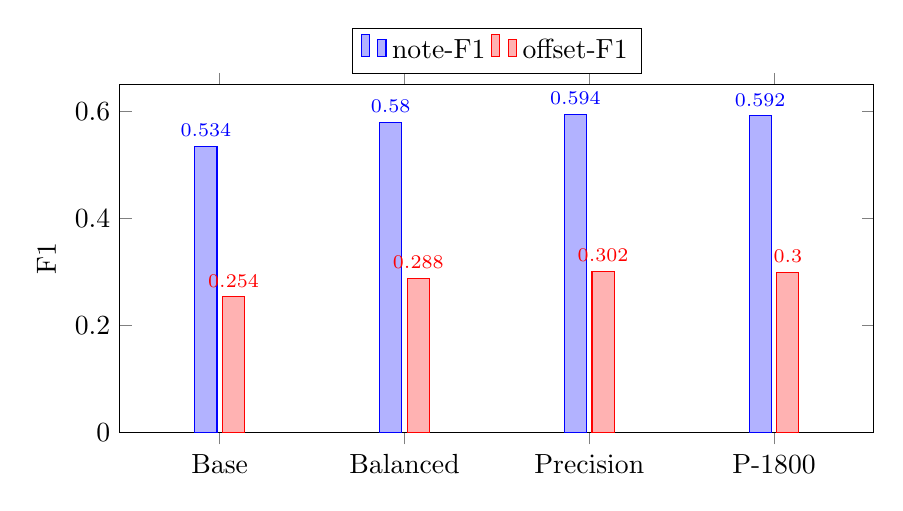
\begin{tikzpicture}
\begin{axis}[
    ybar,
    width=0.92\linewidth,
    height=6cm,
    ymin=0,
    ymax=0.65,
    ylabel={F1},
    symbolic x coords={Base,Balanced,Precision,P-1800},
    xtick=data,
    bar width=8pt,
    enlarge x limits=0.18,
    legend style={at={(0.5,1.03)},anchor=south,legend columns=2},
    nodes near coords,
    nodes near coords style={font=\scriptsize,/pgf/number format/fixed,/pgf/number format/precision=3},
]
\addplot coordinates {(Base,0.5344) (Balanced,0.5799) (Precision,0.5942) (P-1800,0.5919)};
\addplot coordinates {(Base,0.2538) (Balanced,0.2880) (Precision,0.3016) (P-1800,0.2995)};
\legend{note-F1, offset-F1}
\end{axis}
\end{tikzpicture}
\caption{候选系统在 \code{val\_calib512} 上的 note-F1 与 offset-F1。Base、Balanced、Precision 和 P-1800 分别对应表 \ref{tab:amt_metrics} 中的四个候选设置。}
\label{fig:amt_metrics_bar}
\end{figure}


图 \ref{fig:calibration_tradeoff} 更直接地展示了这一校准现象。高 precision 设置提高了误检控制，但 recall 与 \code{pred/ref} 同时下降，说明系统进入欠生成状态。对于谱面生成任务，欠生成会造成漏音和和弦缺音；过生成则会带来短假音和声部碰撞。因此，最佳事件级候选并不一定是最高 precision 设置，而应在 F1、recall 和 \code{pred/ref} 之间取得稳定平衡。

\begin{figure}[H]
\centering
\begin{tikzpicture}
\begin{axis}[
    ybar,
    width=0.92\linewidth,
    height=6cm,
    ymin=0,
    ymax=1.05,
    ylabel={数值},
    symbolic x coords={Base,Balanced,Precision,P-1800},
    xtick=data,
    bar width=7pt,
    enlarge x limits=0.18,
    legend style={at={(0.5,1.03)},anchor=south,legend columns=3},
]
\addplot coordinates {(Base,0.5400) (Balanced,0.5932) (Precision,0.6916) (P-1800,0.6897)};
\addplot coordinates {(Base,0.5288) (Balanced,0.5671) (Precision,0.5208) (P-1800,0.5184)};
\addplot coordinates {(Base,0.9793) (Balanced,0.9561) (Precision,0.7531) (P-1800,0.7517)};
\legend{precision, recall, pred/ref}
\end{axis}
\end{tikzpicture}
\caption{precision、recall 与 \code{pred/ref} 的校准权衡。高 precision 设置提高误检控制，但候选音规模明显偏低。}
\label{fig:calibration_tradeoff}
\end{figure}


\subsection{参数规模、训练目标与长音恢复}

RQ2 检查模型容量变化是否稳定带来性能提升。表 \ref{tab:version_comparison} 将最终候选按系统角色归纳。均衡候选和高置信候选具有相同参数规模，但表现出不同的校准特性：前者更接近参考音符规模，后者在 precision 和 offset-F1 上较强，同时产生明显欠生成。这说明模型容量不是唯一决定因素，训练目标、样本分布和阈值校准会改变模型的错误类型。

\begin{table}[H]
\centering
\caption{最终候选设置及实验角色}
\label{tab:version_comparison}
\begin{tabularx}{\textwidth}{l l l X}
\toprule
候选设置 & 参数量 & 实验角色 & 结果解释 \\
\midrule
v13\_best & 64.89M & 保守候选 & 谱面干净，候选音规模接近参考；主要不足是漏音和和弦缺音。 \\
v15\_best & 171.33M & 均衡候选 & note-F1、recall 与候选音规模较均衡，适合作为演奏 MIDI 与数值分析主候选。 \\
v19\_selected & 171.33M & 高置信候选 & 误检控制和 offset 较好，但候选音规模偏低；适合作为长音与高置信补音辅助。 \\
v13+v19 hybrid & 组合模型 & 混合修正候选 & 以保守候选维持谱面稳定，并在上下文支撑下补充和弦与长音；尚无同口径 full-val 固化记录。 \\
\bottomrule
\end{tabularx}
\end{table}


长音指标进一步支持这一结论。高置信候选在 0.5--2 秒 duration ratio 上高于均衡候选，说明其对部分长音或 offset 候选具有辅助价值；但其 chord note recall 和完整和弦率下降，难以直接作为展示谱主输出。因此，本文将高置信候选定位为辅助信息源，不把它作为完整替代模型。该现象也与 ByteDance 高分辨率钢琴转录强调 offset 与踏板建模的方向一致 \cite{kong2021highres}，但本系统仍受训练规模与校准策略限制。

\subsection{谱面可读性与事件密度的张力}

RQ3 关注谱面整理层是否改善 MusicXML 可读性。表 \ref{tab:demo_metrics} 给出了 Test\_new 的展示谱指标。所有候选输出均能生成可打开的 MusicXML，长音连线率为 1.0，说明谱面层在输出合法性和长音连线方面已经稳定。差异主要集中在 chord verticality、score/performance note ratio 和 voice collision 上。

\begin{table}[H]
\centering
\caption{Test\_new 展示谱质量指标}
\label{tab:demo_metrics}
\begin{tabular}{lrrrrrr}
\toprule
输出 & perf notes & score notes & score/perf & rests & chord vert. & collisions \\
\midrule
v13 score & 514 & 607 & 1.181 & 2 & 0.384 & 7 \\
v13+v15 hybrid & 585 & 702 & 1.200 & 2 & 0.447 & 12 \\
v13+v19 hybrid & 598 & 714 & 1.194 & 2 & 0.462 & 13 \\
v15 score & 1425 & 1775 & 1.246 & 0 & 0.840 & 154 \\
v19 score & 1233 & 1518 & 1.231 & 0 & 0.763 & 73 \\
\bottomrule
\end{tabular}

\vspace{2mm}
\footnotesize 数据来源：\code{outputs/demo\_compare/final\_demo\_report.json}。chord vert. 为和弦垂直性指标，collisions 为声部碰撞计数。
\end{table}


图 \ref{fig:score_quality_tradeoff} 显示，高密度候选具有较高 chord verticality，但 voice collision 也显著增加。保守候选的声部碰撞最低，但和弦垂直性不足，反映出和弦缺音和对齐不足。混合修正候选在保持低可见休止符和低碰撞的同时提高 chord verticality，说明受上下文约束的补音机制能够改善部分和弦结构。该结果与 PM2S 和 Score Transformer 的结论相呼应：可听 MIDI 与可读乐谱之间存在结构性差异，谱面层需要独立评价 \cite{liu2022pm2s,suzuki2021scoretransformer}。

\begin{figure}[H]
\centering
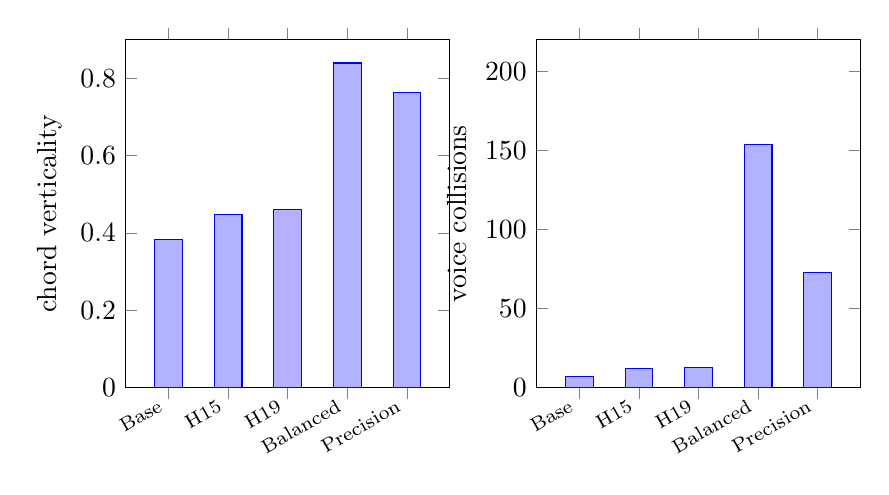
\begin{tikzpicture}
\begin{groupplot}[
    group style={group size=2 by 1, horizontal sep=1.1cm},
    width=0.47\linewidth,
    height=6cm,
    ybar,
    symbolic x coords={Base,H15,H19,Balanced,Precision},
    xtick=data,
    x tick label style={rotate=30,anchor=east,font=\scriptsize},
    enlarge x limits=0.18,
]
\nextgroupplot[
    ymin=0,
    ymax=0.9,
    ylabel={chord verticality},
]
\addplot coordinates {(Base,0.384) (H15,0.447) (H19,0.462) (Balanced,0.840) (Precision,0.763)};
\nextgroupplot[
    ymin=0,
    ymax=220,
    ylabel={voice collisions},
]
\addplot coordinates {(Base,7) (H15,12) (H19,13) (Balanced,154) (Precision,73)};
\end{groupplot}
\end{tikzpicture}
\caption{Test\_new 展示谱中的和弦垂直性与声部碰撞。高密度候选提高垂直音组比例，同时显著增加声部碰撞；混合修正在两者之间取得折中。}
\label{fig:score_quality_tradeoff}
\end{figure}


\subsection{错误类型与消融结论}

RQ4 关注混合修正和谱面层对具体错误的作用。最终结果可归纳为四类错误。第一，弱音伴奏、密集和弦内部音和快速琶音仍会造成漏音；保守候选谱面干净，但音乐结构可能不完整。第二，长音截断需要同时观察 offset-F1、duration ratio 和 truncated rate；高置信候选在部分长音分桶上更好，但候选音规模偏小。第三，和弦拆散与错位表现为 chord verticality 下降；高密度候选虽然改善垂直性，却会增加 voice collision。第四，冗余休止符已明显减少，但声部方向、左右手分配和乐句层级仍依赖规则。

表 \ref{tab:convergence_lessons} 总结了收束阶段的主要消融结论。实验表明，继续扩大参数量并不能单独解决谱面质量问题；高召回或高 precision 设置都需要经过阈值校准和谱面整理。混合修正的有效位置主要集中在和弦缺音、低音长音和重复长音延展。当辅助候选脱离局部上下文时，补音会转化为短假音和谱面污染。因此，当前系统更适合采用“稳定主候选 + 受限辅助修正 + 独立谱面层”的组合。

\begin{table}[H]
\centering
\caption{收束阶段的主要消融结论}
\label{tab:convergence_lessons}
\begin{tabularx}{\textwidth}{l X X}
\toprule
现象 & 观察 & 结论 \\
\midrule
继续增大模型 & v15/v19 均为 171.33M，但 v19 虽 F1 略高，\code{pred/ref} 只有 0.753。 & 参数规模不是唯一瓶颈，阈值、训练目标和数据分布会决定模型是过生成还是欠生成。 \\
直接用高候选谱面 & v15/v19 直接谱面 chord verticality 高，但 voice collision 明显上升。 & 高 recall MIDI 不能直接等同于可读 MusicXML，必须有独立谱面层。 \\
只用干净 base & v13 visible rests 和碰撞较低，但和弦垂直性不足。 & 过度保守会产生漏音和和弦缺音，需要上下文约束的补音机制。 \\
hybrid rescue & v13+v19 在 Test\_new 上提高 chord verticality，同时保持 rests 为 2。 & 辅助模型应只在和弦、长音和重复长音延长等受支持场景中介入。 \\
\bottomrule
\end{tabularx}
\end{table}


总体来看，本文系统与外部强钢琴 AMT 模型仍有差距。ByteDance 系统在 MAESTRO 上报告了 96.72\% onset F1 \cite{kong2021highres}，而本文报告的是 full validation note-F1、offset-F1、\code{pred/ref} 与 MusicXML 指标，二者口径不同。该差距说明后续仍需加强高分辨率 onset/offset 回归、踏板建模和更大规模训练；同时，谱面质量还需要吸收 performance-MIDI-to-score 方向的学习式 beat、voice 和 notation 建模 \cite{liu2022pm2s,beyer2024midi2score}。

\section{讨论}

\subsection{与外部强基线的关系}

ByteDance 高分辨率钢琴转录在 MAESTRO 上报告了 96.72\% 的 onset F1 \cite{kong2021highres}，显著高于本项目当前的 note-F1。这个差距是真实存在的，但不能简单地把两个数字直接等同。外部结果通常针对标准钢琴 AMT benchmark，并使用成熟训练规模、精细 onset/offset 回归和踏板建模。本项目报告的是 dense-AMT 收束体系下的 full validation note-F1、offset-F1、\code{pred/ref} 以及 MusicXML 谱面质量指标。二者评价目标不同。

这种差距也给出后续优化方向。如果继续追求 AMT 指标，需要进一步吸收高分辨率 onset/offset 回归和踏板建模，而不能单纯扩大 backbone。当前 v19 的表现已经说明，大参数模型如果没有足够稳定的数据、目标和校准，可能转向高 precision 欠生成，最终不利于谱面生成。

\subsection{谱面质量的独立性}

项目中最直接的工程教训是，MIDI 可听不代表 MusicXML 可读。演奏 MIDI 保留细微 timing 和持续状态是合理的，但乐谱需要被组织为拍点、声部和小节。早期输出中大量不明休止符、长音误断和和弦拆散，主要来自把 performance note events 直接填入单声部谱面。后续将谱面层独立出来后，visible rests 已显著下降，MusicXML 可打开性稳定，但和弦分配和声部碰撞仍需改进。

\subsection{系统价值与表述边界}

MiniMT3-Piano 的价值主要体现在完整、可调试、可展示的系统闭环。系统经历了从 seq2seq 到 dense AMT、从单一 F1 到双目标输出、从纯后处理到 hybrid rescue 的迭代。最终系统能够给出明确推理入口、模型选择原则、指标报告和 MusicXML 输出，为后续扩展和人工校订提供基础。

同时，论文表述需要保持边界清楚。本文不将规则谱面层包装成通用 MIDI-to-score 模型，也不把 Test\_new 个例的展示改善泛化为全数据集结论。系统贡献主要体现在工程整合、错误分析和面向场景的评价设计。

\section{局限性与未来工作}

当前系统仍存在四类局限。第一，note-F1 与 offset-F1 距离强钢琴 AMT 系统仍有明显差距，尤其是在弱音、密集和弦和复杂踏板场景下。第二，v19 虽然提高了 precision 和 offset，但 \code{pred/ref} 偏低，说明其不能直接承担完整转录任务。第三，谱面层仍主要是规则与启发式方法，无法像人类一样理解乐句结构和左右手惯用写法。第四，本文缺少系统的人类主观评价，展示谱质量主要由自动指标和局部目检支撑。

未来工作可以沿三条小而准的路线推进。第一，对 v19 assistant 做 pitch-aware calibration 和更细粒度阈值选择，将其 \code{pred/ref} 从 0.753 拉近到 0.85--0.95，同时保持 precision。第二，继续优化 hybrid rescue，只补有音乐上下文支持的和弦缺音和低音长音，避免孤立短音进入谱面。第三，借鉴 PM2S 与 Score Transformer，引入轻量 performance-MIDI-to-score 模块，学习声部、拍点和记谱结构，而不仅依赖规则后处理。

\section{结论}

本文总结了 MiniMT3-Piano 的系统架构、训练流程、解码策略、谱面生成方法和最终收束结果。系统最终选择 dense AMT 作为主线，保留演奏 MIDI 与展示 MusicXML 两类输出，并在收束阶段确定 v15 作为数值指标主模型、v13 作为干净谱面基底、v19 作为高 precision/offset 辅助模型。实验表明，参数规模扩大并不必然带来更好谱面；对于练习与展示场景，合理的阈值校准、onset-gated 解码、hybrid rescue 和独立 score pipeline 同样关键。

总体而言，MiniMT3-Piano 尚未达到领先钢琴 AMT 系统的识别水平，但已经形成了面向展示和练习的完整系统。该系统的主要特色在于把 AMT 指标与谱面质量共同纳入设计目标，并用可复现的脚本、指标和 MusicXML 输出支撑后续优化。

\bibliographystyle{unsrt}
\bibliography{references}

\end{document}
